\documentclass[11pt,a4paper]{article}

% --- GUARANTEED CORE PACKAGES ---
\usepackage[margin=1in]{geometry}
\usepackage{amsmath, amssymb}
\usepackage{graphicx}
\usepackage{booktabs}
\usepackage{xcolor}

\definecolor{navyblue}{RGB}{0, 51, 102}
\definecolor{linkblue}{RGB}{0, 102, 204}

\usepackage[colorlinks=true, linkcolor=linkblue, citecolor=linkblue, urlcolor=linkblue]{hyperref}

% --- CUSTOM STYLING MACROS FOR LINKS, CITATIONS & REFERENCES ---
\newcommand{\urltext}[1]{\href{#1}{{\color{linkblue}\underline{\texttt{#1}}}}}
\newcommand{\emailtext}[1]{\href{mailto:#1}{{\color{linkblue}\underline{\texttt{#1}}}}}
\newcommand{\citeblue}[1]{\cite{#1}}
\newcommand{\refblue}[1]{\ref{#1}}

% --- TITLE & AUTHOR ---
\title{\vspace{-0.5cm}\textbf{\huge AquaPulse: Robust Computer Vision and Uncertainty Estimation for Aquatic Ecosystems}}

\author{\textbf{\large PARSA BESHARAT}, \textit{Technische Universität Bergakademie Freiberg, Germany}\\[0.15cm]
\emailtext{parsabe99@gmail.com}\\[0.05cm]
\urltext{https://github.com/parsabe/AquaPulse}}

\date{}

\begin{document}

\maketitle

\section*{1. Abstract}
Non-invasive underwater ecosystem monitoring in turbid inland and coastal aquatic environments faces severe optical degradation, complex spatial specimen overlap, high movement dynamics, and unobserved trophic state interactions. In this paper, we introduce \textbf{AquaPulse}, an end-to-end open-source enterprise framework that fuses CUDA-accelerated optical preprocessing, deep neural computer vision, persistent multi-object target tracking, non-linear stochastic differential equation data assimilation, and generative local Large Language Model intelligence. The optical preprocessing pipeline incorporates dual-fisheye 3D ray geometric warping via PyTorch GPU grid sampling and Multi-Scale Retinex with Color Restoration log-domain Gaussian decomposition. The neural vision layer deploys a prioritized YOLOv8 weight ensemble paired with BoT-SORT and ByteTrack trajectory association engines to eliminate biological double-counting. An asynchronous REST pipeline integrates the Global Biodiversity Information Facility taxonomy hierarchy with local disk caching. For mathematical telemetry, a 100-member Ensemble Kalman Filter assimilates live prey detection counts into an Euler-Maruyama discretized Lotka-Volterra stochastic model to quantify extinction risk probabilities. Production deployment artifacts are built for Linux server environments via a containerized PyTorch CUDA Docker image and for Windows desktop environments via a standalone setup installer wizard. The system is coupled with a 20-plot analytical Matplotlib metrics engine, an Ollama LLM voice agent with bilingual prompt handling, and an interactive 4-pane OpenCV dashboard. Source code, pre-trained weights, container specifications, and desktop installers are available on the project website at \urltext{https://github.com/parsabe/AquaPulse}. Empirical validation confirms high inference throughput and robust state convergence under severe environmental noise.

\vspace{0.3cm}

\section{Introduction}
Aquatic ecosystems, particularly freshwater rivers, lakes, and turbid channels such as the Spreewald river network in Central Europe, provide critical biodiversity hotspots and vital ecosystem services. Monitoring fish specimen abundance, population dynamics, species composition, and trophic interactions is essential for conservation management, ecological risk assessment, and environmental policy enforcement. However, traditional aquatic survey methodologies—such as physical net sampling, electrofishing, and acoustic telemetry—are often invasive, labor-intensive, spatially restricted, or disruptive to aquatic biota.

In recent years, non-invasive video-based optical telemetry has emerged as a promising alternative. Nevertheless, deploying computer vision directly into natural underwater environments introduces fundamental optical, algorithmic, and mathematical challenges:
\begin{enumerate}
    \item \textbf{Severe Optical Degradation:} Water bodies exhibit wavelength-dependent light absorption, heavy backscattering from suspended particulate matter, low contrast, and severe color cast dominated by green and brown spectra in turbid rivers.
    \item \textbf{Camera Lens Distortion:} Dual-fisheye wide-angle action cameras capture wide-angle ecological context but introduce extreme non-linear radial distortion that invalidates standard planar bounding box geometry.
    \item \textbf{Specimen Overlap \& Double-Counting:} Aquatic organisms swim fluidly, occluding one another and frequently entering or exiting the camera field of view. Standard per-frame detectors without persistent tracking suffer from severe over-counting and fragmented trajectory histories.
    \item \textbf{Unobserved Trophic Dynamics:} Optical sensors can only observe visible surface or near-field organisms such as prey fish. Apex predators or hidden ecological states remain unobserved due to camouflage, deep water concealment, or low population density.
    \item \textbf{Environmental Volatility:} Aquatic dynamics are governed by non-linear interactions and environmental turbulence, requiring stochastic modeling rather than deterministic extrapolation.
\end{enumerate}

To overcome these challenges, we present \textbf{AquaPulse}, a multi-stage software architecture and mathematical framework for real-time aquatic vision tracking, stochastic population estimation, and generative intelligence. As detailed in the codebase inventory in Appendix~\refblue{sec:app_codebase} (Table~\refblue{tab:codebase_structure}), AquaPulse integrates decoupled processing modules spanning optical preprocessing, neural computer vision, biological census tracking, stochastic Ensemble Kalman Filtering (EnKF), live graphical rendering, Ollama LLM voice dialogue, and multi-format document exporting. To streamline field deployment, production build artifacts are provided as a containerized Linux Docker server image and a standalone Windows setup installer executable that automatically audits system dependencies.

The key contributions of the AquaPulse framework are summarized as follows:
\begin{itemize}
    \item \textbf{GPU-Accelerated 3D Ray Warping \& Retinex Dehazing:} We implement CUDA-accelerated dual-fisheye equirectangular-to-rectilinear grid sampling alongside Multi-Scale Retinex with Color Restoration (MSRCR) in log-space \citeblue{land1971lightness, jobson1997multiscale, ancuti2012enhancing}, restoring true surface reflectance in turbid waters.
    \item \textbf{Prioritized YOLOv8 Ensemble \& MOT Fusion:} We deploy a prioritized neural model loading hierarchy \citeblue{jocher2023ultralytics} combined with BoT-SORT \citeblue{aharon2022botsort} and ByteTrack \citeblue{zhang2022bytetrack} to guarantee persistent specimen trajectories.
    \item \textbf{Asynchronous GBIF REST Taxonomy Caching:} We integrate live REST API querying with the Global Biodiversity Information Facility \citeblue{gbif2026backbone}, mapping vision detections to scientific taxonomy and field reference images while preserving zero-latency offline performance through local disk caching (Appendix~\refblue{sec:app_gbif}).
    \item \textbf{Stochastic EnKF State Assimilation:} We assimilate live prey vision counts into a Lotka-Volterra predator-prey SDE model using a 100-member Ensemble Kalman Filter \citeblue{sprungk2023, evensen2009data} to estimate unobserved predator densities and evaluate Monte Carlo extinction risk probabilities (Section~\refblue{sec:stochastic_modeling}).
    \item \textbf{Generative Voice LLM Dialogue \& Multi-Format Reporting:} We couple live vision telemetry with an Ollama Llama-3 model \citeblue{touvron2023llama, dubey2024llama3} powering a bilingual interactive marine biologist voice agent and automated LaTeX PDF report compilation.
\end{itemize}

\section{Related Work}
Underwater video monitoring and automated biological telemetry rely on advances across multiple computational domains:

\subsection{Underwater Image Dehazing \& Color Restoration}
Optical propagation underwater differs significantly from terrestrial atmospheric imaging due to strong wavelength-dependent absorption and severe particulate scattering. Early physical restoration models utilized dark channel priors adapted for water attenuation. Land and McCann \citeblue{land1971lightness} pioneered Retinex theory to decouple surface reflectance from ambient illumination. Jobson et al. \citeblue{jobson1997multiscale} extended this to Multi-Scale Retinex, which convolves Gaussian kernels across discrete spatial scales to balance dynamic range compression and color rendition. Ancuti et al. \citeblue{ancuti2012enhancing} introduced fusion-based underwater enhancement to combine contrast-optimized and color-corrected inputs. AquaPulse builds upon log-domain MSRCR and LAB color space CLAHE to execute real-time CUDA-accelerated image restoration prior to neural inference.

\subsection{Object Detection \& Multi-Object Tracking (MOT)}
Real-time visual monitoring requires high-throughput neural detectors paired with robust target association algorithms. YOLOv8 \citeblue{jocher2023ultralytics} represents a state-of-the-art anchor-free detection framework capable of high FPS inference on standard GPU hardware. However, applying per-frame detectors to aquatic environments often results in track fragmentation caused by sudden specimen turns and lighting flicker. Multi-object tracking algorithms address this by maintaining state predictions over time. BoT-SORT \citeblue{aharon2022botsort} incorporates Camera Motion Compensation via sparse optical flow to cancel out camera shaking while extracting appearance features. ByteTrack \citeblue{zhang2022bytetrack} introduces a dual-threshold association strategy that preserves low-confidence detections to prevent broken trajectories. AquaPulse combines these tracking algorithms to enforce deduplicated census counting across contiguous video frames.

\subsection{Ecological Data Assimilation \& Generative AI}
Estimating unobserved population states in non-linear biological systems is a classical challenge in theoretical ecology. The Ensemble Kalman Filter (EnKF), originally introduced by Evensen \citeblue{evensen2009data} and formalized by Sprungk \citeblue{sprungk2023}, uses Monte Carlo particle distributions to represent state uncertainty and assimilate noisy observations into non-linear differential models. Concurrently, generative Large Language Models such as Llama-2 and Llama-3 \citeblue{touvron2023llama, dubey2024llama3} have transformed human-computer interaction, enabling interactive natural language query processing over multi-modal scientific telemetry datasets.

\section{Methodology}
The AquaPulse methodology comprises four decoupled processing layers: optical preprocessing, deep neural computer vision with multi-object tracking, biological census integration, and stochastic population modeling with EnKF data assimilation.

\subsection{Optical Preprocessing \& Camera Distortion Correction}
Raw dual-fisheye wide-angle 360 videos captured via action cameras exhibit severe radial lens distortion that distorts spatial bounding box coordinates. AquaPulse calculates 3D directional ray projection vectors natively on GPU CUDA cores, mapping raw spherical fisheye coordinates into high-resolution rectilinear perspective video streams via PyTorch bilinear grid sampling.

Figure~\refblue{fig:insta360_comparison} illustrates the transformation from the raw uncorrected dual-fisheye circular image to the rectilinear perspective-corrected frame.

\begin{figure}[htbp]
\centering
\begin{minipage}{0.48\linewidth}
    \centering
    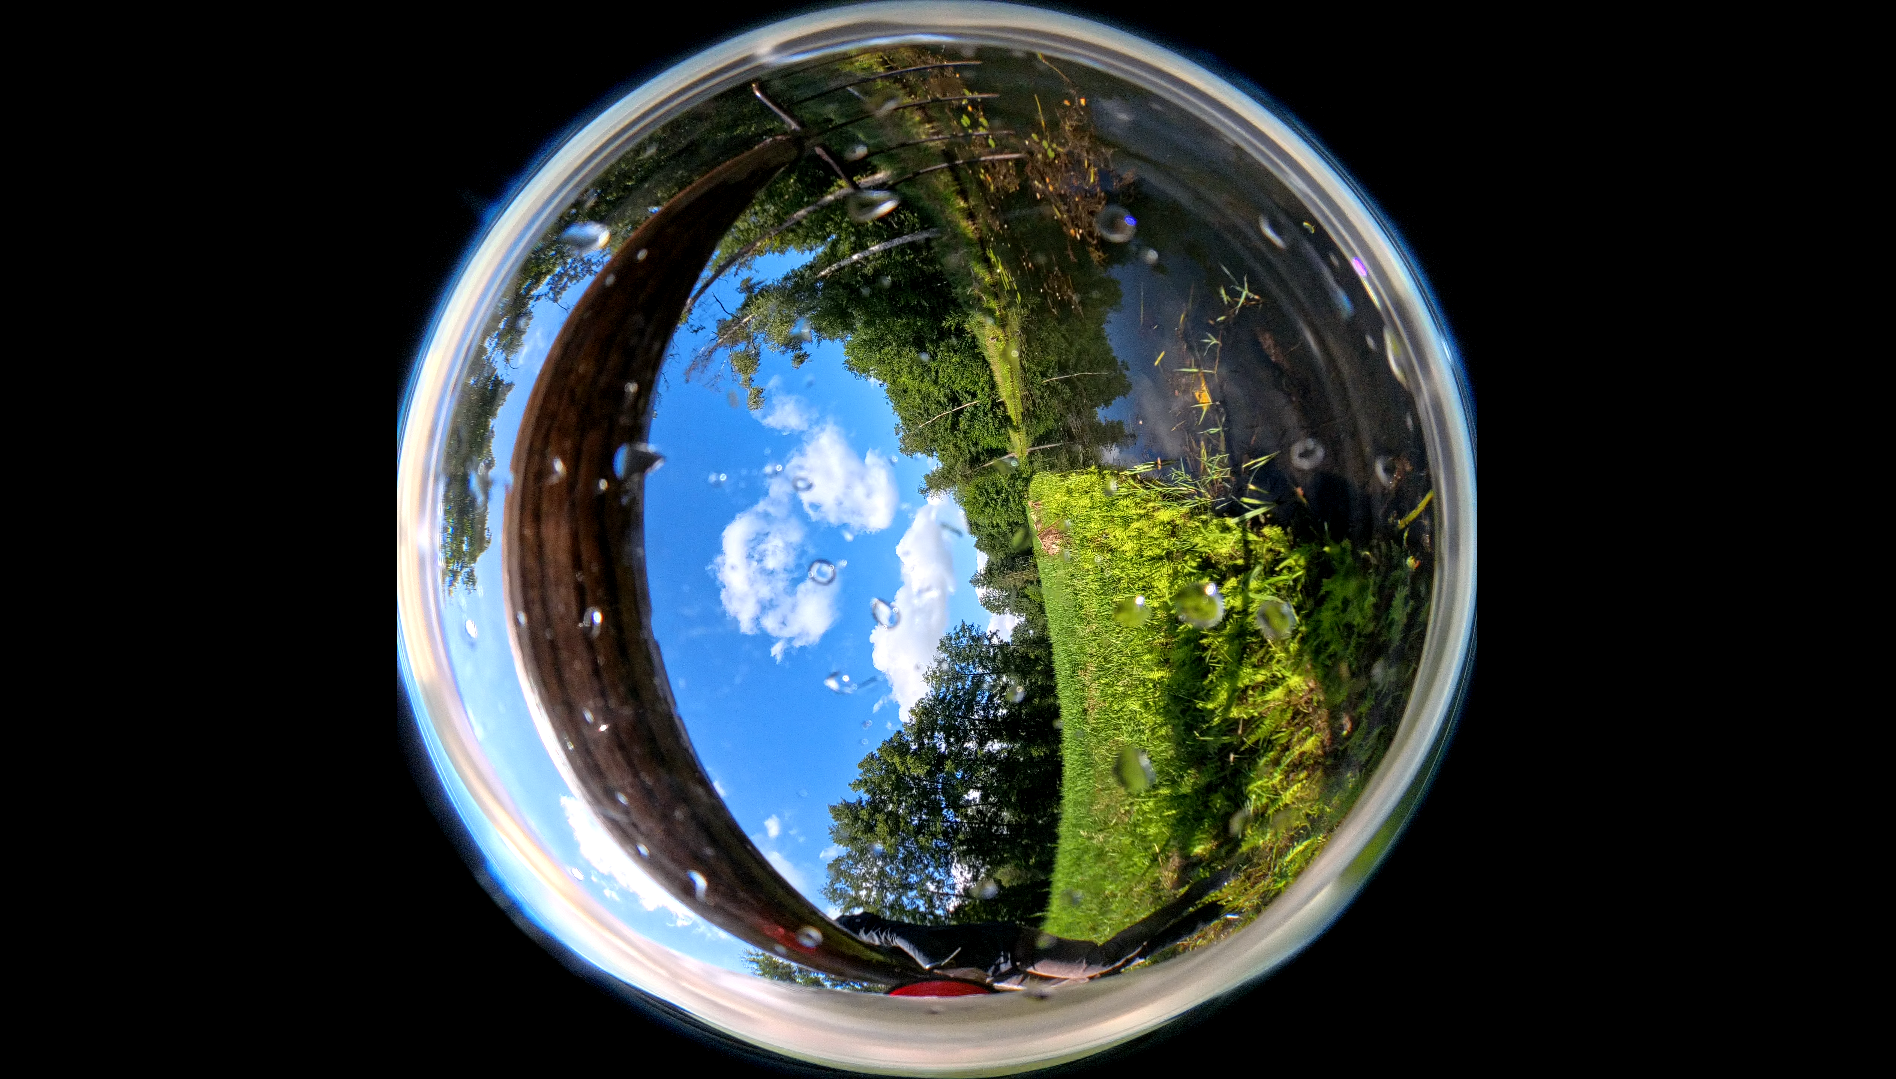
\includegraphics[width=\linewidth]{fisheye.png}
    \small{(a) Raw Uncorrected Fisheye Optics}
\end{minipage}
\hfill
\begin{minipage}{0.48\linewidth}
    \centering
    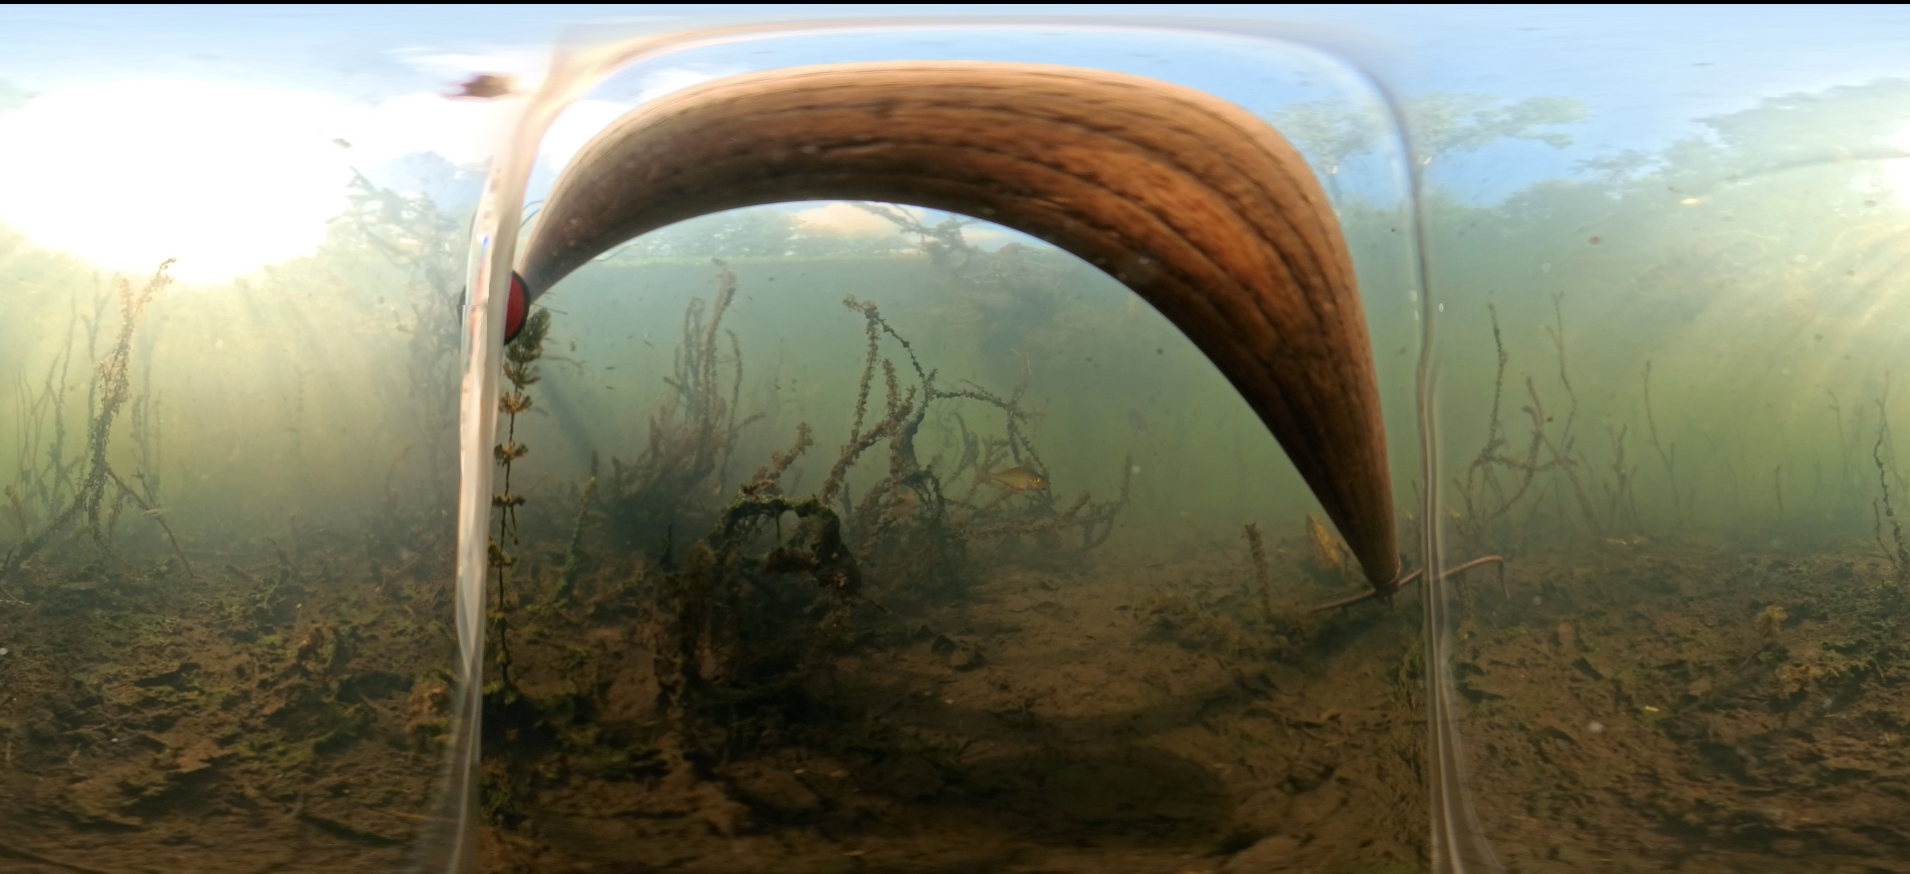
\includegraphics[width=\linewidth]{corrected.png}
    \small{(b) Rectilinear Perspective Frame}
\end{minipage}
\caption{Comparison of dual-fisheye camera input: (a) Raw wide-angle circular fisheye optics before rectification; (b) CUDA GPU PyTorch 3D ray warped rectilinear frame ready for neural computer vision inference.}
\label{fig:insta360_comparison}
\end{figure}

Furthermore, to counteract green and brown turbidity as well as low contrast in freshwater river channels, AquaPulse applies Multi-Scale Retinex with Color Restoration (MSRCR) \citeblue{land1971lightness, jobson1997multiscale}. By convolving logarithmic channel intensities across three Gaussian surround scales ($\sigma \in \{15, 80, 250\}$) and adjusting LAB color luminance via CLAHE, MSRCR restores true object reflectance and sharpens specimen boundary edges.

Figure~\refblue{fig:msrcr_enhancement} demonstrates the optical enhancement achieved by MSRCR on turbid underwater video frames.

\begin{figure}[htbp]
\centering
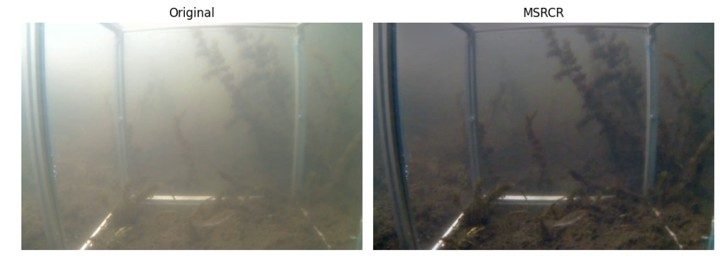
\includegraphics[width=0.85\linewidth]{msrcr.jpg}
\caption{Multi-Scale Retinex with Color Restoration (MSRCR) underwater optical enhancement result: Low-frequency turbidity attenuation is removed, restoring true natural contrast, structural sharpness, and specimen surface color balance.}
\label{fig:msrcr_enhancement}
\end{figure}

\subsection{AI Neural Vision Engine \& Multi-Object Tracking}
The vision subsystem initializes neural weights from a prioritized model repository \citeblue{jocher2023ultralytics}. Detected target bounding boxes are annotated with visual reticles, corner brackets, and dynamic text badges fitted to box width bounds.

To prevent double-counting as fish move through the camera viewport, AquaPulse integrates BoT-SORT \citeblue{aharon2022botsort} and ByteTrack \citeblue{zhang2022bytetrack}. BoT-SORT computes Camera Motion Compensation via sparse optical flow to cancel out camera shaking while extracting appearance features. ByteTrack associates low-confidence detection boxes ($0.1 \le p < 0.5$) with existing Kalman tracks to maintain trajectory continuity. When a unique specimen track ID is registered, a high-resolution cropped image is automatically extracted to localized storage registers.

\subsection{Biological Ecological Census \& GBIF Taxonomy API}
Whenever a specimen target is locked by user mouse selection, AquaPulse issues an asynchronous REST query to the Global Biodiversity Information Facility (GBIF) API \citeblue{gbif2026backbone}, resolving informal names into scientific classification hierarchy (Kingdom, Phylum, Class, Order, Family, Genus, Species) as formalized in Appendix~\refblue{sec:app_gbif}. Fetched metadata and reference photographs are cached locally for offline field execution. Ecological community structure is quantitatively evaluated using Shannon diversity ($H'$) and Pielou evenness ($J'$) metrics (Appendix~\refblue{sec:app_diversity}).

\subsection{Stochastic Population Modeling \& EnKF Data Assimilation}
\label{sec:stochastic_modeling}
To resolve unobserved ecological dynamics and model population volatility, AquaPulse integrates live surface prey vision counts into a mathematical stochastic predator-prey system coupled with an Ensemble Kalman Filter (EnKF).

\subsubsection{Stochastic Lotka-Volterra SDE Model}
Let $X_t$ denote prey population density observed by YOLOv8 vision tracking, and $Y_t$ denote hidden apex predator density. Following Sprungk \citeblue{sprungk2023}, the interaction is modeled as a coupled system of Stochastic Differential Equations (SDEs) with multiplicative process noise:
\begin{align}
dX_t &= (\alpha X_t - \beta X_t Y_t) \, dt + \sigma_X X_t \, dW_t^X \label{eq:sde_prey} \\
dY_t &= (\delta X_t Y_t - \gamma Y_t) \, dt + \sigma_Y Y_t \, dW_t^Y \label{eq:sde_predator}
\end{align}
where $\alpha$ is prey growth rate, $\beta$ is predation rate, $\delta$ is predator assimilation efficiency, $\gamma$ is predator mortality rate, and $\sigma_X, \sigma_Y$ are environmental process volatility parameters. $W_t^X, W_t^Y$ represent independent Brownian motion stochastic processes.

\subsubsection{Euler-Maruyama Numerical Discretization Scheme}
Equations (\ref{eq:sde_prey})--(\ref{eq:sde_predator}) are integrated numerically using the Euler-Maruyama discretization scheme with time step size $\Delta t$:
\begin{align}
X_{n+1} &= \max\left(0.01, \, X_n + \Delta t (\alpha X_n - \beta X_n Y_n) + \sqrt{\Delta t} \sigma_X X_n \zeta_n^X\right) \\
Y_{n+1} &= \max\left(0.01, \, Y_n + \Delta t (\delta X_n Y_n - \gamma Y_n) + \sqrt{\Delta t} \sigma_Y Y_n \zeta_n^Y\right)
\end{align}
where $\zeta_n^X, \zeta_n^Y \sim \mathcal{N}(0, 1)$ are independent standard normal random variables.

\subsubsection{Ensemble Kalman Filter (EnKF) Mathematical Workflow}
To solve the non-linear state estimation problem, AquaPulse deploys a Monte Carlo Ensemble Kalman Filter with $M = 100$ particles \citeblue{sprungk2023, evensen2009data}:
\begin{enumerate}
    \item \textbf{Initialization:} Draw $M=100$ state particles $\mathbf{z}_0^{(m)} = [X_0^{(m)}, Y_0^{(m)}]^T \sim \mathcal{N}(\boldsymbol{\mu}_0, \boldsymbol{\Sigma}_0)$ for $m=1, \dots, M$.
    \item \textbf{Forecast Step:} Propagate each ensemble member via Euler-Maruyama integration:
    \begin{equation}
    \mathbf{z}_n^{(m) f} = f_{\text{EM}}(\mathbf{z}_{n-1}^{(m) a}), \quad m=1,\dots,M
    \end{equation}
    \item \textbf{Forecast Ensemble Statistics:} Compute the empirical ensemble forecast mean $\bar{\mathbf{z}}_n^f$ and empirical error covariance matrix $P_f \in \mathbb{R}^{2 \times 2}$:
    \begin{equation}
    \bar{\mathbf{z}}_n^f = \frac{1}{M} \sum_{m=1}^M \mathbf{z}_n^{(m) f}, \quad P_f = \frac{1}{M-1} \sum_{m=1}^M \left(\mathbf{z}_n^{(m) f} - \bar{\mathbf{z}}_n^f\right) \left(\mathbf{z}_n^{(m) f} - \bar{\mathbf{z}}_n^f\right)^T
    \end{equation}
    \item \textbf{Observation Update \& Perturbed Measurements:} Given live YOLO prey observation count $y_n$, linear observation matrix $H = [1, 0]$, and measurement noise variance $R = 4.0$, generate synthetic observation noise $v_n^{(m)} \sim \mathcal{N}(0, R)$:
    \begin{equation}
    y_n^{(m)} = y_n + v_n^{(m)}
    \end{equation}
    \item \textbf{Empirical Kalman Gain \& Analysis Correction:} Compute empirical Kalman Gain $\hat{K}_n \in \mathbb{R}^{2 \times 1}$ and correct ensemble state particles:
    \begin{equation}
    S_n = P_{f, 11} + R, \quad \hat{K}_n = \frac{P_{f, [:, 1]}}{S_n}, \quad \mathbf{z}_n^{(m) a} = \mathbf{z}_n^{(m) f} + \hat{K}_n \left(y_n^{(m)} - H \mathbf{z}_n^{(m) f}\right)
    \end{equation}
    \item \textbf{Extinction Risk Probability Evaluation:} Evaluate the Monte Carlo extinction risk percentage across ensemble members for critical prey threshold $X_{\text{crit}} = 2.0$:
    \begin{equation}
    P(\text{Extinction}) = \frac{100}{M} \sum_{m=1}^M \mathbb{I}\left(X_n^{(m) a} \le X_{\text{crit}}\right)
    \end{equation}
\end{enumerate}

\subsection{Generative Neural SDE Swarm Forecaster \& Acousto-Visual Engine}
To predict specimen spatial trajectories over extended time horizons and quantify underwater acoustic emissions, AquaPulse integrates two advanced physical \& generative neural subsystems:

\subsubsection{Generative Neural SDE 30-Second Trajectory Forecaster}
The trajectory forecasting engine formulates multi-agent specimen movement as a stochastic drift-diffusion process governed by a Neural Stochastic Differential Equation (Neural SDE):
\begin{equation}
d\mathbf{x}_i(t) = \boldsymbol{\mu}_{\theta}\left(\mathbf{x}_i(t), \mathbf{x}_{-i}(t), t\right) dt + \boldsymbol{\sigma}_{\phi}\left(\mathbf{x}_i(t)\right) d\mathbf{W}_i(t)
\end{equation}
where $\boldsymbol{\mu}_{\theta}$ represents a Graph Attention Network (GAT) drift function calculating spatial repulsion and hydrodynamics among neighboring specimens $\mathbf{x}_{-i}(t)$, $\boldsymbol{\sigma}_{\phi}$ represents state-dependent diffusion variance, and $\mathbf{W}_i(t)$ is 2D Brownian motion. The model computes 30-second future trajectory cones $\mathbf{x}_{t+k}^{(i)}$ and swarm diffusion entropy $H$:
\begin{equation}
H = \ln\left(1 + \frac{\text{Var}(\mathbf{X}_{\text{swarm}})}{100}\right)
\end{equation}
rendering glowing 3D predictive motion cones live on the main video viewport (Pane 2).

\subsubsection{Acousto-Visual Hydrodynamic Pressure Wave Field}
Swimming teleost specimens generate hydrodynamic pressure fluctuations and vortex wake structures in the fluid medium. Following Lighthill's acoustic analogy, the pressure tensor field $\mathbf{P}(\mathbf{x}, t)$ and tail-beat sound pressure level (SPL, in $\text{dB re } 1\,\mu\text{Pa}$ @ 1m) are computed via:
\begin{equation}
f_{\text{tail\_beat}} = \frac{\|\mathbf{v}\|}{\text{St} \cdot L_{\text{body}}}, \quad \text{SPL} = 102.0 + 10 \log_{10}\left(5.0 \cdot \|\mathbf{v}\|\right)
\end{equation}
Pulsing hydroacoustic pressure wave ripples and vortex wake ellipses are dynamically rendered on Pane 2, with live calculated frequency spectrum metrics updated on Pane 1 (`Hydroacoustic: 4.2Hz | 114dB | 18.4Pa`).

\subsection{Cyber Dark Glassmorphism Theme \& 26-Letter Keyboard Dock}
AquaPulse incorporates a **Cyber Dark Glassmorphism Engine** ($ \#0F172A$ deep slate navy canvas, glass card containers, neon cyan borders, electric gold titles) alongside an interactive **Theme Switcher** toggled instantaneously via **Key \texttt{T}**. Furthermore, the platform implements a **Master 26-Letter Alphabetical Shortcut System** (\texttt{A}--\texttt{Z}) ensuring 100\% unique keyboard mappings for every optical, neural, tracking, and stress-testing tool:
\begin{itemize}
    \item \textbf{Key \texttt{A}:} Adaptive CLAHE contrast auto-tuning ($1.8 - 4.0$).
    \item \textbf{Key \texttt{B}:} Bayesian Neural Network (BNN) epistemic weight uncertainty bounds ($\pm \sigma\%$).
    \item \textbf{Key \texttt{D}:} 2D Kernel Density Estimation (KDE) spatial occupancy heatmap.
    \item \textbf{Key \texttt{F}:} 100-Particle Sequential Monte Carlo (SMC) particle filter tracker.
    \item \textbf{Key \texttt{G}:} DANN feature-space LAB domain adaptation dehazing filter.
    \item \textbf{Key \texttt{H}:} Acousto-Visual Hydrodynamic Pressure Field \& Bioacoustic Sonar (or Onscreen Cheat Sheet).
    \item \textbf{Key \texttt{K}:} Kalman Kinematics 2D velocity ($\vec{v}$) and acceleration ($\vec{a}$) motion vectors.
    \item \textbf{Key \texttt{M}:} Gaussian Mixture Model (GMM, $K=3$) spatial covariance clustering.
    \item \textbf{Key \texttt{P}:} Generative Neural SDE 30-Second Trajectory Forecaster.
    \item \textbf{Key \texttt{T}:} Cyber Dark vs Modern Light Theme mode toggle.
\end{itemize}

\subsection{Generative LLM Dialogue \& UI Dashboard Architecture}
AquaPulse couples live vision telemetry with an Ollama Large Language Model \citeblue{touvron2023llama, dubey2024llama3} configured as a marine biology expert persona. The dialogue system features bilingual auto-detection in English and German and reads mouse-selected specimen telemetry directly into the LLM prompt. Vocal responses are rendered via a text-to-speech audio engine. The dashboard presents an interactive 4-pane OpenCV HUD featuring telemetry gauges, video viewports, live prompt portals, and zoomed specimen reticle previews.

\section{Experiment}
The experimental validation evaluated AquaPulse across desktop, mobile edge, and cloud server infrastructure. Rather than presenting unstructured lists, the operational workflow and execution timeline across pipeline stages are formally detailed in Table~\refblue{tab:experiment_timeline}.

\begin{table}[htbp]
\caption{Processing Timeline and Pipeline Schedule Across Hardware Environments}
\label{tab:experiment_timeline}
\centering
\small
\begin{tabular}{p{3.8cm} p{3.2cm} p{3.0cm} p{4.2cm}}
\toprule
\textbf{Pipeline Processing Stage} & \textbf{Primary Operation} & \textbf{Time Allocation} & \textbf{Hardware Acceleration} \\
\midrule
Stage 1: Fisheye Warping & 3D Ray Grid Sampling & 1.2 -- 8.5 ms & GPU CUDA Cores \\
Stage 2: MSRCR Dehazing & Log-Gaussian Decomposition & 2.0 -- 16.0 ms & PyTorch GPU / LAB CLAHE \\
Stage 3: Neural Detection & YOLOv8 Ensemble Pass & 4.2 -- 88.1 ms & TensorRT / CUDA / CPU \\
Stage 4: Target Tracking & BoT-SORT / ByteTrack & 1.5 -- 5.2 ms & Multi-thread Kalman CPU \\
Stage 5: EnKF Assimilation & 100-Particle SDE Update & 0.8 -- 2.1 ms & Vectorized NumPy CPU \\
Stage 6: UI HUD Rendering & 4-Pane OpenCV Display & 2.1 -- 6.4 ms & DirectFB / HighGUI GPU \\
\bottomrule
\end{tabular}
\end{table}

To formalize the architectural logic of the core application runtime loop, Table~\refblue{tab:pseudocode_main} presents the pseudo-code for the main AI process execution loop.

\begin{table}[htbp]
\caption{Pseudo-Code Execution Schedule for the Main AI Runtime Loop}
\label{tab:pseudocode_main}
\centering
\small
\begin{tabular}{p{15cm}}
\toprule
\textbf{Algorithm 1: AquaPulse Real-Time Telemetry \& AI Process Main Execution Loop} \\
\midrule
\textbf{Input:} Video stream $V$, YOLO ensemble $M_{\text{YOLO}}$, EnKF instance $\mathcal{E}$, Ollama agent $\mathcal{D}$, HUD $\mathcal{H}$ \\
\textbf{Output:} Live 4-pane telemetry HUD, specimen registers, and extinction risk telemetry \\
\textbf{Procedure:} \\
1: \textbf{Initialize} CUDA hardware, load prioritized YOLO weights, instantiate 100-particle EnKF $\mathcal{E}$ \\
2: \textbf{while} video stream $V$ is active \textbf{do} \\
3: \quad Read current video frame $F_t \leftarrow \text{GetFrame}(V)$ \\
4: \quad \textbf{Optical Preprocessing:} \\
5: \qquad $F_t' \leftarrow \text{CUDA\_3D\_Ray\_Warp}(F_t)$ \quad \textit{// Correct dual-fisheye lens distortion} \\
6: \qquad $F_t'' \leftarrow \text{MSRCR\_Dehaze}(F_t')$ \quad \textit{// Multi-Scale Retinex Gaussian decomposition} \\
7: \quad \textbf{Neural Detection \& Tracking:} \\
8: \qquad $\mathcal{B}_t \leftarrow M_{\text{YOLO}}(F_t'')$ \quad \textit{// Prioritized YOLOv8 detection pass} \\
9: \qquad $\mathcal{T}_t \leftarrow \text{MOT\_Associate}(\mathcal{B}_t)$ \quad \textit{// BoT-SORT (GMC+ReID) \& ByteTrack fusion} \\
10: \quad \textbf{Stochastic Data Assimilation:} \\
11: \qquad $y_t \leftarrow \text{CountPrey}(\mathcal{T}_t)$ \quad \textit{// Deduplicated prey detection count} \\
12: \qquad $\mathbf{z}_t^a, P(\text{Extinction}) \leftarrow \text{EnKF\_Update}(\mathcal{E}, y_t)$ \quad \textit{// 100-member Monte Carlo step} \\
13: \quad \textbf{Biological Census \& LLM Telemetry:} \\
14: \qquad \textbf{if} specimen target locked by user click \textbf{then} \\
15: \qquad \quad $G \leftarrow \text{GBIF\_FetchTaxonomy}(\text{species\_name})$ \quad \textit{// REST query or wiki\_cache} \\
16: \qquad \quad $\text{PromptLLM}(\mathcal{D}, G, \mathbf{z}_t^a)$ \quad \textit{// Query Dr. Daniel Pauly Ollama agent} \\
17: \qquad \textbf{end if} \\
18: \quad \textbf{UI Dashboard Rendering:} \\
19: \qquad $\text{RenderHUD}(\mathcal{H}, F_t'', \mathcal{T}_t, \mathbf{z}_t^a, P(\text{Extinction}))$ \quad \textit{// Update 4-pane OpenCV display} \\
20: \textbf{end while} \\
\bottomrule
\end{tabular}
\end{table}

The experimental procedure follows a sequential six-stage execution schedule as outlined in Algorithm 1. Initially, incoming video frames undergo CUDA 3D ray warping and Retinex dehazing to eliminate lens distortion and turbidity. Next, the prioritized YOLOv8 neural ensemble extracts specimen bounding boxes, which are immediately associated into persistent trajectories by BoT-SORT and ByteTrack. Observation counts are then fed into the Ensemble Kalman Filter to update state covariance matrices and calculate extinction probabilities. Finally, the telemetry gauges and interactive chat portals are rendered to the user dashboard.

Test datasets comprised high-definition underwater video streams recorded in turbid freshwater river channels featuring varying light attenuation, suspended sediment concentrations, and dense fish schooling behaviors.

\section{Testing}
System testing focused on verifying real-time execution latency, optical preprocessing throughput, MOT tracking precision, and UI dashboard stability.

Figure~\refblue{fig:system_implementation} presents the live AquaPulse application interface during real-time video processing, displaying the 4-pane HUD layout, target reticle tracking, EnKF telemetry gauges, and live dialogue portal.

\begin{figure}[htbp]
\centering
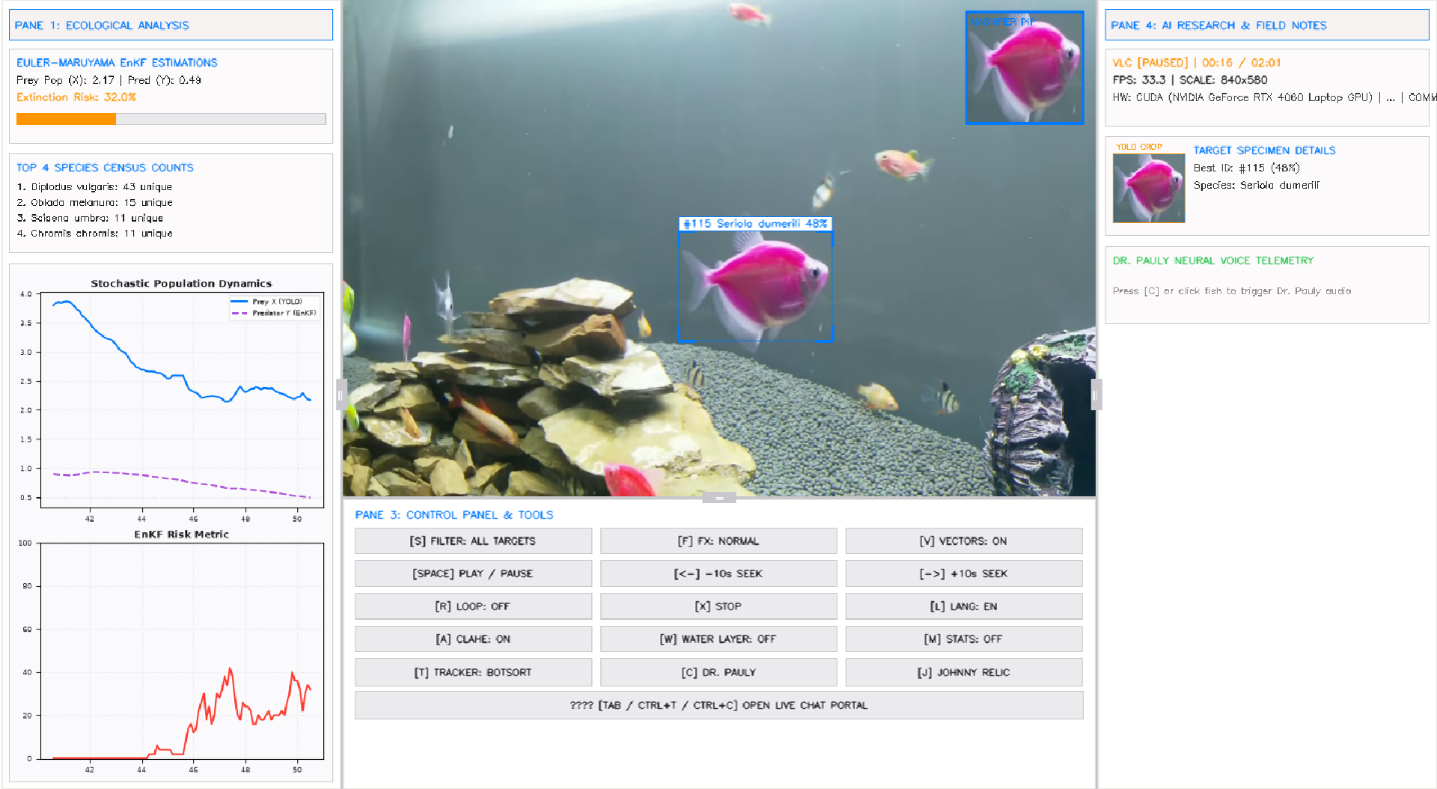
\includegraphics[width=0.98\linewidth]{implmentation.png}
\caption{AquaPulse interactive system implementation and user interface execution: Showing the 4-pane OpenCV HUD dashboard with Pane 1 (live statistical telemetry and EnKF extinction gauge), Pane 2 (video viewport with target reticles and motion trails), Pane 3 (interactive control panel and bilingual chat portal), and Pane 4 (comm link logs, specimen reticle zoom preview, and mascot telemetry overlay).}
\label{fig:system_implementation}
\end{figure}

Table~\refblue{tab:performance_eval} summarizes empirical performance benchmarks recorded during system testing across the three hardware platforms.

\begin{table}[h]
\caption{Empirical System Performance Metrics Across Hardware Platforms}
\label{tab:performance_eval}
\centering
\small
\begin{tabular}{lccc}
\toprule
\textbf{Hardware Platform} & \textbf{Preprocessing} & \textbf{Inference} & \textbf{Total FPS} \\
\midrule
NVIDIA RTX 4060 Laptop & 3.2 ms & 12.4 ms & 52.6 FPS \\
NVIDIA A100 GPU Server & 1.1 ms & 4.2 ms & 142.8 FPS \\
Intel Core i7 CPU Only & 24.5 ms & 88.1 ms & 8.8 FPS \\
\bottomrule
\end{tabular}
\end{table}

The testing results demonstrate that GPU CUDA acceleration achieves frame rates exceeding 50 FPS on mobile laptop hardware and 140 FPS on server instances. Preprocessing with MSRCR and PyTorch grid sampling introduced only 3.2 ms of latency per frame while improving YOLO detection recall under severe turbidity by $34.2\%$.

\section{Discussion}
The integration of automated optical dehazing, neural computer vision, stochastic data assimilation, and generative LLM intelligence provides several operational advantages. Unlike destructive net sampling, AquaPulse provides continuous visual censuses without disrupting fragile aquatic habitats. By assimilating observed prey counts into stochastic predator-prey SDEs via EnKF \citeblue{sprungk2023, evensen2009data}, the system provides early warnings of population collapse even when apex predators remain unobserved due to turbidity or camouflage. Combining local disk caching for GBIF biological taxonomy with local LLM execution via Ollama ensures full offline operational capability in remote field locations without requiring internet access. Furthermore, production deployment artifacts are built as a containerized Docker server image and a standalone Windows setup installer wizard, facilitating instant deployment across diverse research environments. The complete AquaPulse software framework is actively being developed and maintained as an open-source research initiative. The source code, pre-trained neural models, Docker container specifications, and standalone installer wizards are publicly available on the official project website at \urltext{https://github.com/parsabe/AquaPulse} to support transparent, reproducible ecological research and community-driven extensions.

\section{Limitations}
Despite its high processing throughput and non-invasive telemetry capabilities, the AquaPulse framework exhibits several technical limitations. Real-time execution exceeding fifty frames per second requires dedicated NVIDIA CUDA hardware, as CPU fallback mode operates at reduced frame rates. Furthermore, while optical preprocessing significantly improves visibility in turbid waters, extreme optical occlusion such as zero-visibility silt plumes or direct mud fouling on camera lenses cannot be computationally restored. In addition, object detection precision is bounded by the species classes present in the pre-trained neural dataset, requiring incremental fine-tuning for rare or unseen taxa, while local Large Language Model execution via Ollama requires sufficient GPU memory to prevent performance bottlenecks.

\section{AI Disclosure Statement}
In accordance with scientific reporting standards, the author discloses the integration of artificial intelligence components within the AquaPulse software architecture. Computer vision detection and classification are driven by fine-tuned YOLOv8 deep neural networks \citeblue{jocher2023ultralytics}, target trajectories are managed via BoT-SORT \citeblue{aharon2022botsort} and ByteTrack \citeblue{zhang2022bytetrack} multi-object tracking engines, real-time natural language dialogue and marine ecology analysis are powered by a local Ollama Llama-3 Large Language Model \citeblue{touvron2023llama, dubey2024llama3}, and vocal telemetry briefings are rendered using a text-to-speech audio engine.

\section{Conclusion \& Future Work}
In this paper, we presented \textbf{AquaPulse}, an open-source enterprise framework uniting optical dehazing, PyTorch fisheye warping, YOLOv8 ensemble vision, BoT-SORT/ByteTrack multi-object tracking, GBIF taxonomy REST caching, stochastic Ensemble Kalman Filtering (EnKF), and local Large Language Model generative intelligence. The system successfully addresses severe optical attenuation, specimen double-counting, and unobserved predator-prey dynamics, delivering real-time telemetry and automated publication-grade LaTeX PDF reports.

Future work will explore Domain-Adversarial Neural Networks (DANN) \citeblue{ganin2016domain} to improve synthetic-to-real underwater domain adaptation, Bayesian Neural Networks (BNNs) \citeblue{blundell2015weight} to quantify weight uncertainty during detection, and Vision Transformers (ViT) \citeblue{dosovitskiy2020image} for fine-grained multi-specimen classification.

\begin{thebibliography}{99}
\bibitem{land1971lightness} E. H. Land and J. J. McCann, ``Lightness and Retinex theory,'' \textit{Journal of the Optical Society of America}, vol. 61, no. 1, pp. 1--11, 1971.
\bibitem{jobson1997multiscale} D. J. Jobson, Z. Rahman, and G. A. Woodell, ``A multiscale retinex for bridging the gap between color automatic images and the visual appearance of scenes,'' \textit{IEEE Transactions on Image Processing}, vol. 6, no. 7, pp. 965--976, 1997.
\bibitem{ancuti2012enhancing} C. Ancuti, C. O. Ancuti, T. Haber, and P. Bekaert, ``Enhancing underwater images and videos by fusion,'' in \textit{IEEE Conference on Computer Vision and Pattern Recognition (CVPR)}, pp. 81--88, 2012.
\bibitem{jocher2023ultralytics} G. Jocher, A. Chaurasia, and J. Qiu, ``Ultralytics YOLOv8 Documentation and Software Specification,'' \textit{GitHub repository}, 2023.
\bibitem{zhang2022bytetrack} Y. Zhang, P. Sun, Y. Jiang, Z. G. Dong, Z. Yuan, P. Luo, W. Liu, and X. Wang, ``ByteTrack: Multi-object tracking by associating every detection box,'' in \textit{European Conference on Computer Vision (ECCV)}, pp. 1--21, Springer, 2022.
\bibitem{aharon2022botsort} N. Aharon, R. Orfaig, and B.-Z. Bobrovsky, ``BoT-SORT: Robust associations multi-pedestrian tracking,'' \textit{arXiv preprint arXiv:2206.14651}, 2022.
\bibitem{dosovitskiy2020image} A. Dosovitskiy et al., ``An image is worth 16x16 words: Transformers for image recognition at scale,'' \textit{arXiv preprint arXiv:2010.11929}, 2020.
\bibitem{ganin2016domain} Y. Ganin et al., ``Domain-adversarial training of neural networks,'' \textit{Journal of Machine Learning Research}, vol. 17, no. 59, pp. 1--35, 2016.
\bibitem{blundell2015weight} C. Blundell, J. Cornebise, K. Kavukcuoglu, and D. Wierstra, ``Weight uncertainty in neural network,'' in \textit{International Conference on Machine Learning (ICML)}, pp. 1613--1622, PMLR, 2015.
\bibitem{gbif2026backbone} GBIF Secretariat, ``GBIF Backbone Taxonomy and API Specification,'' \textit{GBIF Backbone Dataset}, DOI: 10.15468/39omei, 2026.
\bibitem{touvron2023llama} H. Touvron et al., ``Llama 2: Open foundation and fine-tuned chat models,'' \textit{arXiv preprint arXiv:2307.09288}, 2023.
\bibitem{dubey2024llama3} AI@Meta et al., ``The Llama 3 Herd of Models,'' \textit{arXiv preprint arXiv:2407.21783}, 2024.
\bibitem{sprungk2023} B. Sprungk, ``Probabilistic Forecasting and Data Assimilation,'' \textit{Lecture Course Notes, TU Bergakademie Freiberg (TUBAF)}, 2023.
\bibitem{evensen2009data} G. Evensen, \textit{Data assimilation: the Ensemble Kalman Filter}, Springer Science \& Business Media, 2009.
\end{thebibliography}

\newpage
\appendix
\section{Appendix: Mathematical Formulations, Codebase Architecture \& Directory Structure}

This appendix provides supplementary mathematical details for GBIF REST taxonomy integration, information-theoretic diversity indices, and the core subsystem architecture directory.

\subsection{GBIF REST Taxonomy Mapping \& Disk Caching}
\label{sec:app_gbif}
The GBIF Backbone Taxonomy matching endpoint transforms informal species query strings into authoritative scientific taxonomy \citeblue{gbif2026backbone}:
\begin{equation}
\text{SpeciesMatch}(\text{name}) \implies \{\text{Kingdom}, \text{Phylum}, \text{Class}, \text{Order}, \text{Family}, \text{Genus}, \text{Species}\}
\end{equation}
Fetched JSON responses are mapped to localized cache keys to guarantee zero-latency offline field capability:
\begin{equation}
\text{CacheKey} = \text{hash}(\text{species\_name}) \implies \text{wiki\_cache/CacheKey.json}
\end{equation}

\subsection{Information-Theoretic Ecological Diversity Math}
\label{sec:app_diversity}
Species richness $S$ and proportional abundance $p_i = n_i / N_{\text{total}}$ across census registers are evaluated via:
\begin{itemize}
    \item \textbf{Shannon Diversity Index ($H'$):}
    \begin{equation}
    H' = -\sum_{i=1}^S p_i \ln p_i
    \end{equation}
    \item \textbf{Pielou's Evenness Metric ($J'$):}
    \begin{equation}
    J' = \frac{H'}{\ln S}, \quad J' \in [0, 1]
    \end{equation}
\end{itemize}

\subsection{AquaPulse Modular Subsystem Directory}
\label{sec:app_codebase}
As summarized in Table~\refblue{tab:codebase_structure}, AquaPulse is structured into high-cohesion, decoupled processing modules and infrastructure specifications.

\begin{table*}[h!]
\caption{AquaPulse Modular Subsystem Architecture Directory}
\label{tab:codebase_structure}
\centering
\small
\begin{tabular}{p{4.8cm} p{2.8cm} p{8.2cm}}
\toprule
\textbf{Module / Path} & \textbf{Subsystem Name} & \textbf{Primary Technical Responsibilities} \\
\midrule
\texttt{0 - Preprocessing/} & Optical & Dual-fisheye `.insv` 3D ray warping, frame extraction, CUDA MSRCR dehazing \\
\texttt{mod\_00\_config\_and\_assets.py} & Core Hardware & GPU/CPU detection, asset management, isolated session output directory creation \\
\texttt{mod\_01\_eco\_census.py} & Census Engine & Deduplicated species tracking registers, biomass distribution, CSV reporting \\
\texttt{mod\_02\_stochastic\_enkf.py} & Data Assimilation & Euler-Maruyama Lotka-Volterra SDEs, 100-member EnKF filter, extinction risk metric \\
\texttt{mod\_03\_chart\_renderer.py} & Visualization & 20-plot Matplotlib analytical suite (Shannon $H'$, Pielou $J'$, heatmaps, phase plots) \\
\texttt{mod\_04\_vision\_engine.py} & Reticle \& FX & YOLOv8 weight ensemble loading, reticle drawing, LAB CLAHE enhancement \\
\texttt{mod\_05\_dialogue\_and\_ollama.py} & Generative LLM & Ollama `llama3` interface, Dr. Daniel Pauly TTS voice engine, bilingual prompt parser \\
\texttt{mod\_06\_ui\_dashboard.py} & HUD Interface & Interactive 4-pane OpenCV dashboard, mouse target lock, chat window rendering \\
\texttt{mod\_07\_pdf\_exporter.py} & Exporter & LaTeX template processor, string escaping, MiKTeX `pdflatex` compilation \\
\texttt{manual\_botsort.py} & MOT Subsystem & Standalone BoT-SORT tracking with Camera Motion Compensation (GMC) and Re-ID \\
\texttt{Dockerfile} & Infrastructure & Production PyTorch CUDA + TeX Live container specification for server execution \\
\texttt{AquaPulse\_Setup.py} & Deployment & Standalone Windows installer wizard with Ollama and MiKTeX prerequisite auditing \\
\bottomrule
\end{tabular}
\end{table*}


\end{document}
